\section{ПОЛУЧЕНИЕ ОПИСАНИЙ NPC}

Хоть получение диалогов NPC является необходимым первым шагом в создании набора данных для моделирования диалогов, этого недостаточно, если учесть важность имитации ответов NPC в наборе данных. Анализ доступных инструментов модификации игр для Infinity Engine показал, что преобразование имен файлов диалогов в соответствующие символы, отображаемые в игре, требует логики, специфичной для игры, а получение имен персонажей из имен файлов диалогов с помощью обычных инструментов весьма неоднозначно. Чтобы преодолеть эту проблему, были использованы передовые языковые модели для синтеза описаний NPC в определенном формате. Был использован метод Few-Shot, который включал предоставление примеров реплик NPC, содержащих частичные описания NPC. В результате алгоритм получения описаний NPC выглядит следующим образом:
\begin{enumerate}
  \item Все диалоги группируются по имени файла, из которого были получены диалоги NPC с игроком.
  \item Формируются уникальные и упорядочные примеры реплик NPC так, чтобы количество токенов в примерах + количество токенов в инструкции не превышало 512 токенов.
  \item Примеры реплик вместе с инструкцией отправляются в виде запроса на сервер, обслуживающий модель.
  \item Полученный ответ записывается в файл формата <<.csv>> в виде filename, description.
\end{enumerate}

Все эксперименты были выполнены на потребительском оборудовании, включающем 32 Гб оперативной памяти, 20-ядерный процессор и графический процессор NVIDIA RTX 3090Ti с объемом памяти 24 Гб. Поэтому синтез данных не был проводим на оборудовании максимальной мощности, но доступном для исследований. На начало первого квартала 2023 года, одним из наиболее эффективных семейств предобученных моделей для генерации текста по количеству параметров и выходных метрик является LLaMa \cite{llama-paper}. На основе инструкционных данных, было разработано семейство моделей Alpaca \cite{alpaca-docs}, которые достигают качества ответов, сопоставимого с результатами модели ChatGPT \cite{chatgpt-docs}.

Ограничения потребительского оборудовании сказалось и на размере контекста, вмещаемого в модель. Экспериментно было определено, что максимальный размер входной последовательности составляет 512 токенов, а максимальный размер выходной -- 256. В связи с ограничениями на размер входных данных диалог отправляется не весь, а только лишь его часть и при том реплики NPC, потому как в них содержится описание NPC. Было обнаружено, что реплики игрока не влияют на синтезируемое описание NPC, что позволяет экономить размер входных данных. 

Для устойчивого синтеза данных пробовались различные комбинации инструкций и параметров генерации модели. Иногда ответы большой языковой модели не соответствуют требуемому формату, в таком случае стоит пробовать разные подходы к написанию инструкций. Например, использование формулировки <<Сгенерируй данные в формате: ПРИМЕР\_ФОРМАТА>> в отрыве от <<Сгенерируй данные в формате: ПРИМЕР\_ФОРМАТА, НЕ ИСПОЛЬЗУЯ [ПРИМЕР]>>, позволяет получить необходимый ответ с меньшим количеством галлюцинаций и ошибок. Такое поведение можно обосновать тем, что корпус текстов с такими видами формулировок использованный в качестве данных для обучения был больше.

Выгода использования больших языковые моделей для синтеза данных проявляется еще в том, что не для всех NPC написаны описания на таких ресурсах, как wiki и др. Поэтому, используя такой подход, большее количество данных можно покрыть необходимыми описаниями.

В данной работе в качестве инструкции была выбрана следующая: <<Create the personality of a single NPC in DnD style, based on the provided example dialogue in JSON format. Answer in format Name/Alignment/Description/Flaw/Motivation/Personality in a list format written in third person>>. Таким образом были получены описания NPC и датасет DNDD имеет все необходимые компоненты для обучения диалоговой модели.

По данной инструкции были сгенерированы подобные описания: \texttt{\\Name: The Drunk\\
  Alignment: Neutral\\
  Description: A disheveled, stench-ridden waste of a life.\\
  Flaw: Drunk out of his gourd.\\
  Motivation: To get more alcohol.\\
  Personality: The drunk is confused and disoriented, but he is also desperate for more alcohol. He is willing to do anything to get it, even if it means stealing from others.}

\section{АНАЛИЗ DNDD}
Набор данных состоит из 4,5 гигабайт текстовой информации, содержащей в общей сложности 981 тысычу диалогов и 986 миллионов токенов, среди которых 824 миллиона соответствуют ответам NPC. Это составляет 83\% от общего количества токенов. Набор данных также включает 27 миллионов ходов, причем ответы NPC представляют 14 миллионов из них. Примечательно, что некоторые взаимодействия NPC с игроком состоят только из одного предложения. На рисунках \ref{fig:npc-turns-hist}, \ref{fig:pc-turns-hist} отображены распределения частоты диалоговых ходов по длине, а на рисунках \ref{fig:npc-tokens-hist}, \ref{fig:pc-tokens-hist} отображены распределения частоты количества токенов в диалоге по количеству. Наблюдения показывают, что реакция NPC имеет более продолжительную среднюю продолжительность по сравнению с реакцией игрока. Это можно объяснить отличительной особенностью ответов NPC, которая включает в себя хранение дополнительной контекстуальной информации, что приводит к более полному пониманию текущего разговора и, следовательно, к диалогам более высокого качества.
\begin{figure}[H]
  \begin{minipage}{0.48\textwidth}
    \centering
    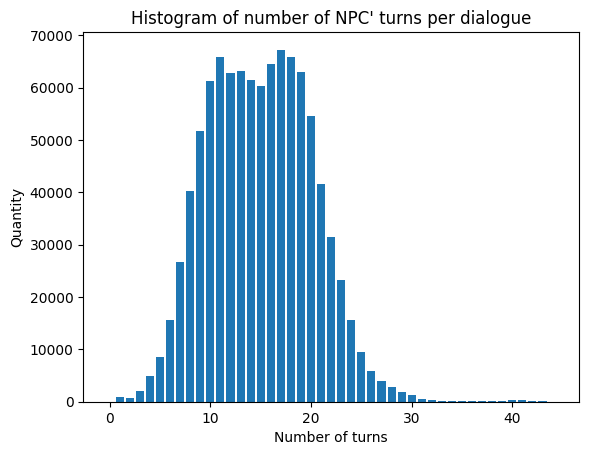
\includegraphics[width=.8\linewidth]{npc-turns-hist}
    \caption{Распределение частоты диалоговых ходов NPC по длине}\label{fig:npc-turns-hist}
  \end{minipage}\hfill
  \begin{minipage}{0.48\textwidth}
    \centering
    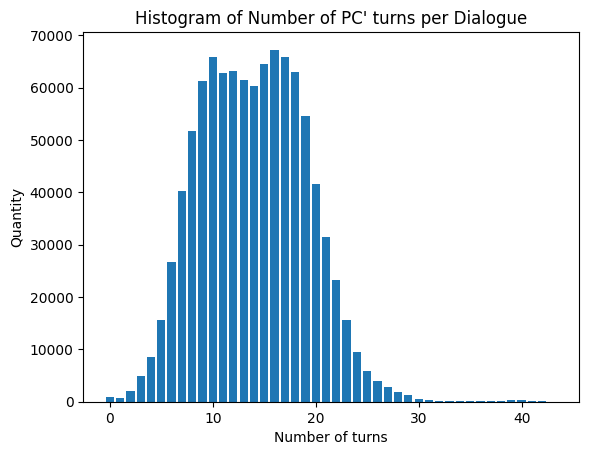
\includegraphics[width=.8\linewidth]{pc-turns-hist}
    \caption{Распределение частоты диалоговых ходов игрока по длине}\label{fig:pc-turns-hist}
  \end{minipage}
\end{figure}

\begin{figure}[H]
  \centering
  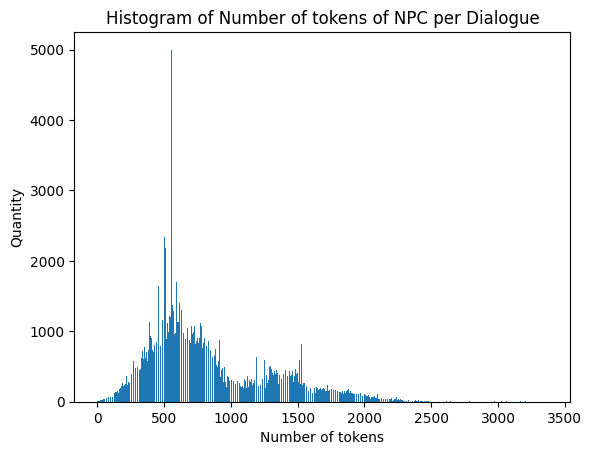
\includegraphics[width=0.6\textwidth]{npc-tokens-hist}
  \caption{Распределение частоты количества токенов в диалоге NPC по количеству}
  \label{fig:npc-tokens-hist}
\end{figure}

\begin{figure}[H]
  \centering
  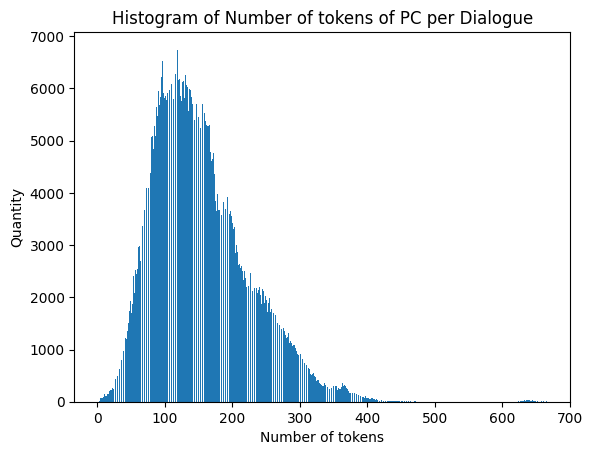
\includegraphics[width=0.6\textwidth]{pc-tokens-hist}
  \caption{Распределение частоты количества токенов в диалоге игрока по количеству}
  \label{fig:pc-tokens-hist}
\end{figure}